\documentclass[border=4pt]{standalone}
\usepackage{tikz}
\usetikzlibrary{arrows,arrows.spaced,positioning}
\begin{document}
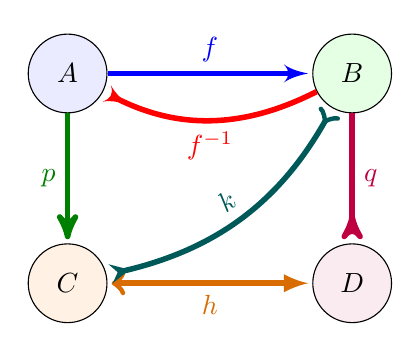
\begin{tikzpicture}[
  node distance=1.65cm and 2.6cm,
  object/.style={draw,circle,minimum size=10mm,inner sep=1pt}
]
  \node[object,fill=blue!8] (A) {$A$};
  \node[object,fill=green!10,right=of A] (B) {$B$};
  \node[object,fill=orange!10,below=of A] (C) {$C$};
  \node[object,fill=purple!8,right=of C] (D) {$D$};

  \draw[blue,line width=2pt,-{spaced latex'}] (A) -- node[above] {$f$} (B);
  \draw[red,line width=2pt,-{spaced latex' reversed}] (B) to[bend left=27] node[below] {$f^{-1}$} (A);
  \draw[green!50!black,line width=2pt,-{spaced stealth'}] (A) -- node[left] {$p$} (C);
  \draw[purple,line width=2pt,-{spaced stealth' reversed}] (B) -- node[right] {$q$} (D);
  \draw[orange!85!black,line width=2pt,{spaced to}-{spaced latex}] (C) -- node[below] {$h$} (D);
  \draw[teal!70!black,line width=2pt,{spaced stealth reversed}-{spaced to reversed}] (C) to[bend right=24] node[above,sloped] {$k$} (B);
\end{tikzpicture}
\end{document}
